\documentclass[aspectratio=169,10pt]{beamer}

% ── Packages ──────────────────────────────────────────────────────────────────
\usepackage[T1]{fontenc}
\usepackage[utf8]{inputenc}
\usepackage{inconsolata}
\usepackage{amsmath}
\usepackage{booktabs}
\usepackage{microtype}
\usepackage{xcolor}
\usepackage{tikz}
\usepackage{array}
\usepackage{colortbl}
\usepackage{graphicx}

% ── Color Palette ─────────────────────────────────────────────────────────────
\definecolor{Navy}{HTML}{0A2540}
\definecolor{Gold}{HTML}{C49A19}
\definecolor{PageBg}{HTML}{FAFAFA}
\definecolor{TableHdr}{HTML}{EEF2F7}
\definecolor{RuleColor}{HTML}{CBD5E1}
\definecolor{BodyText}{HTML}{0A2540}
\definecolor{MutedText}{HTML}{6B7280}
\definecolor{Success}{HTML}{059669}
\definecolor{Danger}{HTML}{DC2626}

% ── Theme Base ────────────────────────────────────────────────────────────────
\usetheme{default}
\setbeamertemplate{navigation symbols}{}
\setbeamercolor{background canvas}{bg=PageBg}
\setbeamercolor{normal text}{fg=BodyText}
\setbeamercolor{frametitle}{fg=white,bg=Navy}
\setbeamercolor{structure}{fg=Navy}
\setbeamercolor{alerted text}{fg=Danger}
\setbeamercolor{block title}{fg=white,bg=Navy}
\setbeamercolor{block body}{fg=BodyText,bg=TableHdr}

% ── Frame Title ───────────────────────────────────────────────────────────────
\setbeamertemplate{frametitle}{%
  \nointerlineskip
  \begin{beamercolorbox}[%
    wd=\paperwidth,ht=2.6ex,dp=1.0ex,%
    leftskip=1.2cm,rightskip=1.2cm]{frametitle}%
    \usebeamerfont{frametitle}\insertframetitle%
  \end{beamercolorbox}%
  \nointerlineskip
  {\color{Gold}\hrule height 1.5pt}%
}

% ── Footline ──────────────────────────────────────────────────────────────────
\setbeamertemplate{footline}{%
  \nointerlineskip
  {\color{RuleColor}\hrule height 0.4pt}%
  \begin{beamercolorbox}[%
    wd=\paperwidth,ht=2.2ex,dp=0.8ex,%
    leftskip=0.8cm,rightskip=0.8cm]{normal text}%
    {\tiny\color{MutedText}\textcopyright{} Shannon Capital --- Confidential}%
    \hfill
    {\tiny\color{MutedText}\insertframenumber\,/\,\inserttotalframenumber}%
  \end{beamercolorbox}%
}

% ── Typography ────────────────────────────────────────────────────────────────
\setbeamerfont{frametitle}{size=\normalsize,series=\bfseries}
\setbeamerfont{title}{size=\LARGE,series=\bfseries}
\setbeamerfont{subtitle}{size=\small,series=\mdseries}
\setbeamersize{text margin left=1.2cm,text margin right=1.2cm}
\setlength{\parskip}{0.45em}
\setlength{\parindent}{0pt}

% ── Metadata ──────────────────────────────────────────────────────────────────
\title{Shannon's Demon}
\subtitle{Strategy Overview --- SOL/BRL Volatility Harvesting}
\author{Shannon Capital}
\date{Backtest Period: Apr 2020 -- May 2026}
\institute{}

\begin{document}

\setbeamercolor{background canvas}{bg=Navy}
\begin{frame}[plain]
\begin{tikzpicture}[remember picture,overlay]
  \fill[Gold] (current page.north west) rectangle ([yshift=-0.18cm]current page.north east);
  \fill[Gold] (current page.south west) rectangle ([yshift=0.09cm]current page.south east);
\end{tikzpicture}
\vspace{1.8cm}
\begin{center}
  {\color{white}\fontsize{26}{32}\selectfont\bfseries Shannon's Demon}\\[0.4cm]
  {\color{Gold}\rule{7cm}{0.6pt}}\\[0.35cm]
  {\color{white!70!black}\normalsize\mdseries Strategy Overview}\\[0.15cm]
  {\color{Gold}\large\bfseries SOL/BRL Volatility Harvesting}\\[0.8cm]
  {\color{white!50!black}\small Shannon Capital}\\[0.15cm]
  {\color{white!35!black}\footnotesize Backtest: Apr~2020 -- May~2026 \quad\textbullet\quad 2{,}239 trading days}\\[0.15cm]
  {\color{white!35!black}\scriptsize Starting capital: R\$100 \quad Final value: R\$2{,}933}
\end{center}
\end{frame}
\setbeamercolor{background canvas}{bg=PageBg}

\setbeamercolor{background canvas}{bg=Navy}
\begin{frame}[plain]
\begin{tikzpicture}[remember picture,overlay]
  \fill[Gold] (current page.north west) rectangle ([yshift=-0.18cm]current page.north east);
  \fill[Gold] (current page.south west) rectangle ([yshift=0.09cm]current page.south east);
\end{tikzpicture}
\vspace{2.5cm}
\begin{center}
  {\color{Gold}\small\bfseries SECTION I}\\[0.3cm]
  {\color{Gold}\rule{6cm}{0.6pt}}\\[0.4cm]
  {\color{white}\fontsize{22}{28}\selectfont\bfseries The Insight}\\[0.35cm]
  {\color{white!60!black}\normalsize Why does rebalancing generate returns?}
\end{center}
\end{frame}
\setbeamercolor{background canvas}{bg=PageBg}

\begin{frame}{The Problem: Volatility as Risk \textit{and} Return}
\vspace{0.4em}
{\small\color{BodyText}
\textbf{The conventional view:} Volatility is risk. Investors seek to minimize it.

\textbf{The alternative view (Shannon, 1961):} Volatility is a raw material.
If the allocation to a volatile asset is rebalanced back to a fixed target after each price move,
the portfolio systematically \textit{buys after dips and sells into rallies} --- extracting a
return premium even when the underlying asset's long-run price is zero.

\vspace{0.5em}
\begin{block}{Key Insight}
A portfolio that rebalances between a volatile asset and cash
can outperform \textbf{both} assets held separately in choppy, mean-reverting markets.
\end{block}

\vspace{0.3em}
SOL/BRL is one of the most volatile major crypto pairs.
With daily absolute returns averaging \textbf{1--3\%}, the rebalancing premium is substantial.
}
\end{frame}

\begin{frame}{Shannon's Demon --- A Brief History}
\vspace{0.4em}
{\small\color{BodyText}
\textbf{Claude Shannon} (1916--2001), inventor of information theory, first described
this portfolio strategy in a 1961 MIT seminar. The name ``Shannon's Demon''
was coined by analogy with Maxwell's Demon --- a thought experiment where an agent
extracts work from a thermal system by exploiting microscopic fluctuations.

\vspace{0.3em}
Shannon showed that a \textbf{continuously rebalanced} 50/50 portfolio between
a stock and cash grows at rate:
\[
  g = \mu - \tfrac{1}{2}\sigma^2 + \tfrac{1}{4}\sigma^2
    = \mu - \tfrac{1}{4}\sigma^2
\]
whereas the unbalanced portfolio grows at $\mu - \tfrac{1}{2}\sigma^2$.
The rebalancing bonus $+\tfrac{1}{4}\sigma^2$ is the \textbf{volatility premium}.

\vspace{0.3em}
\textbf{William Poundstone} popularized the concept in \textit{Fortune's Formula} (2005).
The strategy requires no forecasting ability --- only a commitment to a fixed allocation
and the discipline to rebalance when drift exceeds a threshold.
}
\end{frame}

\begin{frame}{The Intuition: A Round-Trip Thought Experiment}
\vspace{0.2em}
{\small\color{BodyText}
Start with \textbf{R\$10{,}000}: R\$5{,}000 SOL + R\$5{,}000 BRL.
SOL \textbf{doubles}, then returns to its original price.}

\vspace{0.3em}
\arrayrulecolor{RuleColor}
\begin{center}
\begin{tabular}{@{\hspace{0.4em}}l r r r r@{\hspace{0.4em}}}
\toprule
\rowcolor{Navy}\textcolor{white}{\textbf{Step}} &
  \textcolor{white}{\textbf{SOL value}} &
  \textcolor{white}{\textbf{BRL value}} &
  \textcolor{white}{\textbf{Total}} &
  \textcolor{white}{\textbf{Action}} \\
\midrule
Start (SOL @ P)         & R\$5{,}000 & R\$5{,}000 & R\$10{,}000 & --- \\
SOL doubles (@ 2P)      & R\$10{,}000 & R\$5{,}000 & R\$15{,}000 & Sell SOL \\
After rebalance         & R\$7{,}500 & R\$7{,}500 & R\$15{,}000 & 50/50 restored \\
SOL halves (back to P)  & R\$3{,}750 & R\$7{,}500 & \textcolor{Success}{\textbf{R\$11{,}250}} & --- \\
\midrule
\textbf{Without rebalancing} & R\$5{,}000 & R\$5{,}000 & \textbf{R\$10{,}000} & 0\% net \\
\bottomrule
\end{tabular}
\end{center}

\vspace{0.3em}
{\small\color{BodyText}
\textbf{Rebalancing captured R\$1{,}250 (+12.5\%)} on a round trip that left the buy-and-hold investor with zero gain.
The gain scales as $\approx Vr^2/4$ where $r$ is the price swing --- larger swings yield disproportionately more.}
\end{frame}

\setbeamercolor{background canvas}{bg=Navy}
\begin{frame}[plain]
\begin{tikzpicture}[remember picture,overlay]
  \fill[Gold] (current page.north west) rectangle ([yshift=-0.18cm]current page.north east);
  \fill[Gold] (current page.south west) rectangle ([yshift=0.09cm]current page.south east);
\end{tikzpicture}
\vspace{2.5cm}
\begin{center}
  {\color{Gold}\small\bfseries SECTION II}\\[0.3cm]
  {\color{Gold}\rule{6cm}{0.6pt}}\\[0.4cm]
  {\color{white}\fontsize{22}{28}\selectfont\bfseries Mathematical Framework}\\[0.35cm]
  {\color{white!60!black}\normalsize Deriving the volatility premium}
\end{center}
\end{frame}
\setbeamercolor{background canvas}{bg=PageBg}

\begin{frame}{Weight Mechanics \& Trigger Condition}
\vspace{0.2em}
{\small\color{BodyText}Define portfolio variables at time $t$:}

\vspace{0.3em}
\small
\begin{columns}[T]
\begin{column}{0.50\textwidth}
\begin{align*}
  V_s &= \text{SOL balance} \times \text{SOL price} \\
  V_b &= \text{BRL cash balance} \\
  V   &= V_s + V_b \quad\text{(total)} \\[0.4em]
  w   &= \frac{V_s}{V} \quad\text{(SOL weight)} \\[0.4em]
  \delta &= |\,w - 0.5\,| \quad\text{(deviation)} \\[0.4em]
  \tau &= \frac{\text{bps}}{10{,}000} \quad\text{(threshold)}
\end{align*}
\end{column}
\begin{column}{0.46\textwidth}
\vspace{0.4cm}
\begin{block}{Rebalance Trigger}
\centering
$\delta > \tau$
\end{block}
\vspace{0.4em}
{\small\color{BodyText}
\textbf{Direction:}\\
$w > 0.5$: \textcolor{Danger}{SELL SOL}\\
$w < 0.5$: \textcolor{Success}{BUY SOL}

\vspace{0.3em}
\textbf{Example:} threshold~100~bps\\
SOL at 55\% $\Rightarrow$ $\delta = 500$~bps $> \tau$\\
Trade fires.
}
\end{column}
\end{columns}
\end{frame}

\begin{frame}{Critical Price Move to Trigger}
\vspace{0.1em}
{\small\color{BodyText}
From a 50/50 start, let SOL price change by factor $f$.
The new SOL weight and the triggering price factor are:}

\vspace{0.2em}
\small
\begin{columns}[T]
\begin{column}{0.50\textwidth}
\begin{align*}
  w' &= \frac{f}{f+1} \\[0.3em]
  \delta(f) &= \frac{|f-1|}{2(f+1)} \\[0.5em]
  f^*_{\uparrow} &= \frac{1+2\tau}{1-2\tau}
    \quad\text{(trigger up)} \\[0.3em]
  f^*_{\downarrow} &= \frac{1-2\tau}{1+2\tau}
    \quad\text{(trigger down)}
\end{align*}
\end{column}
\begin{column}{0.46\textwidth}
\vspace{0.2em}
\arrayrulecolor{RuleColor}
\begin{tabular}{@{}r r r@{}}
\toprule
\rowcolor{Navy}
  \textcolor{white}{\textbf{bps}} &
  \textcolor{white}{\textbf{SOL up}} &
  \textcolor{white}{\textbf{SOL down}} \\
\midrule
 50 &  +2.0\% &  $-$2.0\% \\
100 &  +4.1\% &  $-$3.9\% \\
200 &  +8.3\% &  $-$7.7\% \\
300 & +12.9\% & $-$11.3\% \\
500 & +22.2\% & $-$18.2\% \\
\bottomrule
\end{tabular}
\vspace{0.3em}

{\scriptsize\color{MutedText}
For small $\tau$: trigger $\approx 4\tau$.\\
At 100~bps, a $\pm$4\% SOL move fires.}
\end{column}
\end{columns}
\end{frame}

\begin{frame}{Trade Size \& the Volatility Premium}
\vspace{0.2em}
{\small\color{BodyText}
\textbf{Trade size:} the BRL amount that exactly restores 50/50:}

\vspace{0.3em}
\small
\begin{columns}[T]
\begin{column}{0.52\textwidth}
\begin{align*}
  \Delta_{\text{BRL}} &= V \cdot (w - 0.5) \\[0.3em]
  &= V \cdot \delta \quad\text{(same formula for both dirs)}
\end{align*}
\vspace{0.2em}
{\small\color{BodyText}
\textbf{Volatility premium per complete price cycle}
(SOL up by $r$, then back to start):}
\begin{align*}
  \Delta V &\approx \frac{V\,r^2}{4} \quad\text{(leading order, small }r\text{)}
\end{align*}
\end{column}
\begin{column}{0.44\textwidth}
\vspace{0.3em}
\arrayrulecolor{RuleColor}
\begin{tabular}{@{}r r@{}}
\toprule
\rowcolor{Navy}
  \textcolor{white}{\textbf{Price swing } $r$} &
  \textcolor{white}{\textbf{Gain per cycle}} \\
\midrule
10\%  & +0.25\% \\
20\%  & +1.0\%  \\
50\%  & +6.25\% \\
100\% & +12.5\% \\
200\% & +33.3\% \\
\bottomrule
\end{tabular}
\vspace{0.3em}

{\scriptsize\color{MutedText}
Gain is \textbf{quadratic} in the swing.\\
Larger oscillations yield\\
disproportionately more profit.}
\end{column}
\end{columns}
\end{frame}

\begin{frame}{Volatility-Adaptive Rebalance Threshold}
\vspace{0.1em}
{\small\color{BodyText}
The threshold $\tau$ is set proportional to recent realized volatility to avoid
over-trading in calm markets while remaining responsive in volatile ones.}

\vspace{0.2em}
\small
\begin{columns}[T]
\begin{column}{0.52\textwidth}
\begin{align*}
  r_i &= \left|\frac{P_i - P_{i-1}}{P_{i-1}}\right|
    \quad\text{(abs. daily return)} \\[0.3em]
  \text{MAD} &= \frac{1}{n{-}1}\sum_{i=1}^{n-1} r_i
    \quad (n{=}31\text{ days}) \\[0.3em]
  \tau_{\text{bps}} &= \text{clamp}\bigl(
    \text{MAD}{\times}10{,}000{\times}1.5,\;50,\;500\bigr)
\end{align*}
\vspace{0.2em}
{\scriptsize\color{MutedText}
Cache refreshed once daily; CDI floor at 50~bps = fee-adjusted minimum;\\
ceiling at 500~bps prevents indefinite non-action in extreme regimes.}
\end{column}
\begin{column}{0.44\textwidth}
\vspace{0.2em}
\arrayrulecolor{RuleColor}
\begin{tabular}{@{}l r r@{}}
\toprule
\rowcolor{Navy}
  \textcolor{white}{\textbf{Regime}} &
  \textcolor{white}{\textbf{MAD}} &
  \textcolor{white}{\textbf{bps}} \\
\midrule
Very calm      & 0.3\% & 50  (floor) \\
Typical crypto & 1.5\% & 225 \\
Volatile       & 2.0\% & 300 \\
Extreme        & $\geq$3.3\% & 500 (ceiling) \\
\bottomrule
\end{tabular}
\vspace{0.2em}

{\scriptsize\color{MutedText}
\textbf{Why proportional to MAD?}\\
At mult~1.5, trigger fires after\\
$\approx$3 typical daily moves\\
accumulate as drift.}
\end{column}
\end{columns}
\end{frame}

\setbeamercolor{background canvas}{bg=Navy}
\begin{frame}[plain]
\begin{tikzpicture}[remember picture,overlay]
  \fill[Gold] (current page.north west) rectangle ([yshift=-0.18cm]current page.north east);
  \fill[Gold] (current page.south west) rectangle ([yshift=0.09cm]current page.south east);
\end{tikzpicture}
\vspace{2.5cm}
\begin{center}
  {\color{Gold}\small\bfseries SECTION III}\\[0.3cm]
  {\color{Gold}\rule{6cm}{0.6pt}}\\[0.4cm]
  {\color{white}\fontsize{22}{28}\selectfont\bfseries Live Implementation}\\[0.35cm]
  {\color{white!60!black}\normalsize SOL/BRL on Mercado Bitcoin}
\end{center}
\end{frame}
\setbeamercolor{background canvas}{bg=PageBg}

\begin{frame}{Live Implementation --- Mercado Bitcoin (SOL/BRL)}
\vspace{0.2em}
\arrayrulecolor{RuleColor}
\small
\begin{columns}[T]
\begin{column}{0.48\textwidth}
\textbf{Execution pipeline}
\begin{itemize}
  \setlength\itemsep{0.12em}
  \item Poll every 15 min (GitHub Actions)
  \item Fetch SOL/BRL spot price
  \item Compute weight \& deviation
  \item Skip if below adaptive threshold
  \item Fetch balances (authenticated)
  \item Place market order (taker, 0.30\%)
  \item Poll order status (3 s intervals, 10 retries)
  \item Record trade, tax event, snapshot
\end{itemize}
\end{column}
\begin{column}{0.48\textwidth}
\textbf{Risk controls}
\begin{itemize}
  \setlength\itemsep{0.12em}
  \item Slippage guard: reject if fill deviates $>$1\% from expected
  \item 2-hour cooldown between rebalances
  \item Dry-run mode (no live orders)
  \item Tax cap: skip SELL if monthly SELL proceeds would exceed R\$35{,}000
  \item Min portfolio size: skip if total $<$R\$200
  \item Min trade size: skip if rebalance $<$R\$20
\end{itemize}
\end{column}
\end{columns}

\vspace{0.3em}
{\scriptsize\color{MutedText}
All state persisted in SQLite (\texttt{shannonfi.db}).
OAuth2 credentials stored in GNOME Keyring (local) or GitHub Secrets (CI).
Source: \texttt{github.com/lucastsantana/shannonfi}.}
\end{frame}

\setbeamercolor{background canvas}{bg=Navy}
\begin{frame}[plain]
\begin{tikzpicture}[remember picture,overlay]
  \fill[Gold] (current page.north west) rectangle ([yshift=-0.18cm]current page.north east);
  \fill[Gold] (current page.south west) rectangle ([yshift=0.09cm]current page.south east);
\end{tikzpicture}
\vspace{2.5cm}
\begin{center}
  {\color{Gold}\small\bfseries SECTION IV}\\[0.3cm]
  {\color{Gold}\rule{6cm}{0.6pt}}\\[0.4cm]
  {\color{white}\fontsize{22}{28}\selectfont\bfseries Backtest: Apr 2020 \textbackslash\{\}textendash\{\} May 2026}\\[0.35cm]
  {\color{white!60!black}\normalsize 2\{,\}239 trading days \textbackslash\{\}textbullet\{\} R\textbackslash\{\}\$100 starting capital}
\end{center}
\end{frame}
\setbeamercolor{background canvas}{bg=PageBg}

\begin{frame}{Cumulative Performance --- Base 100, Log Scale}
\vspace{0.2em}
\begin{center}
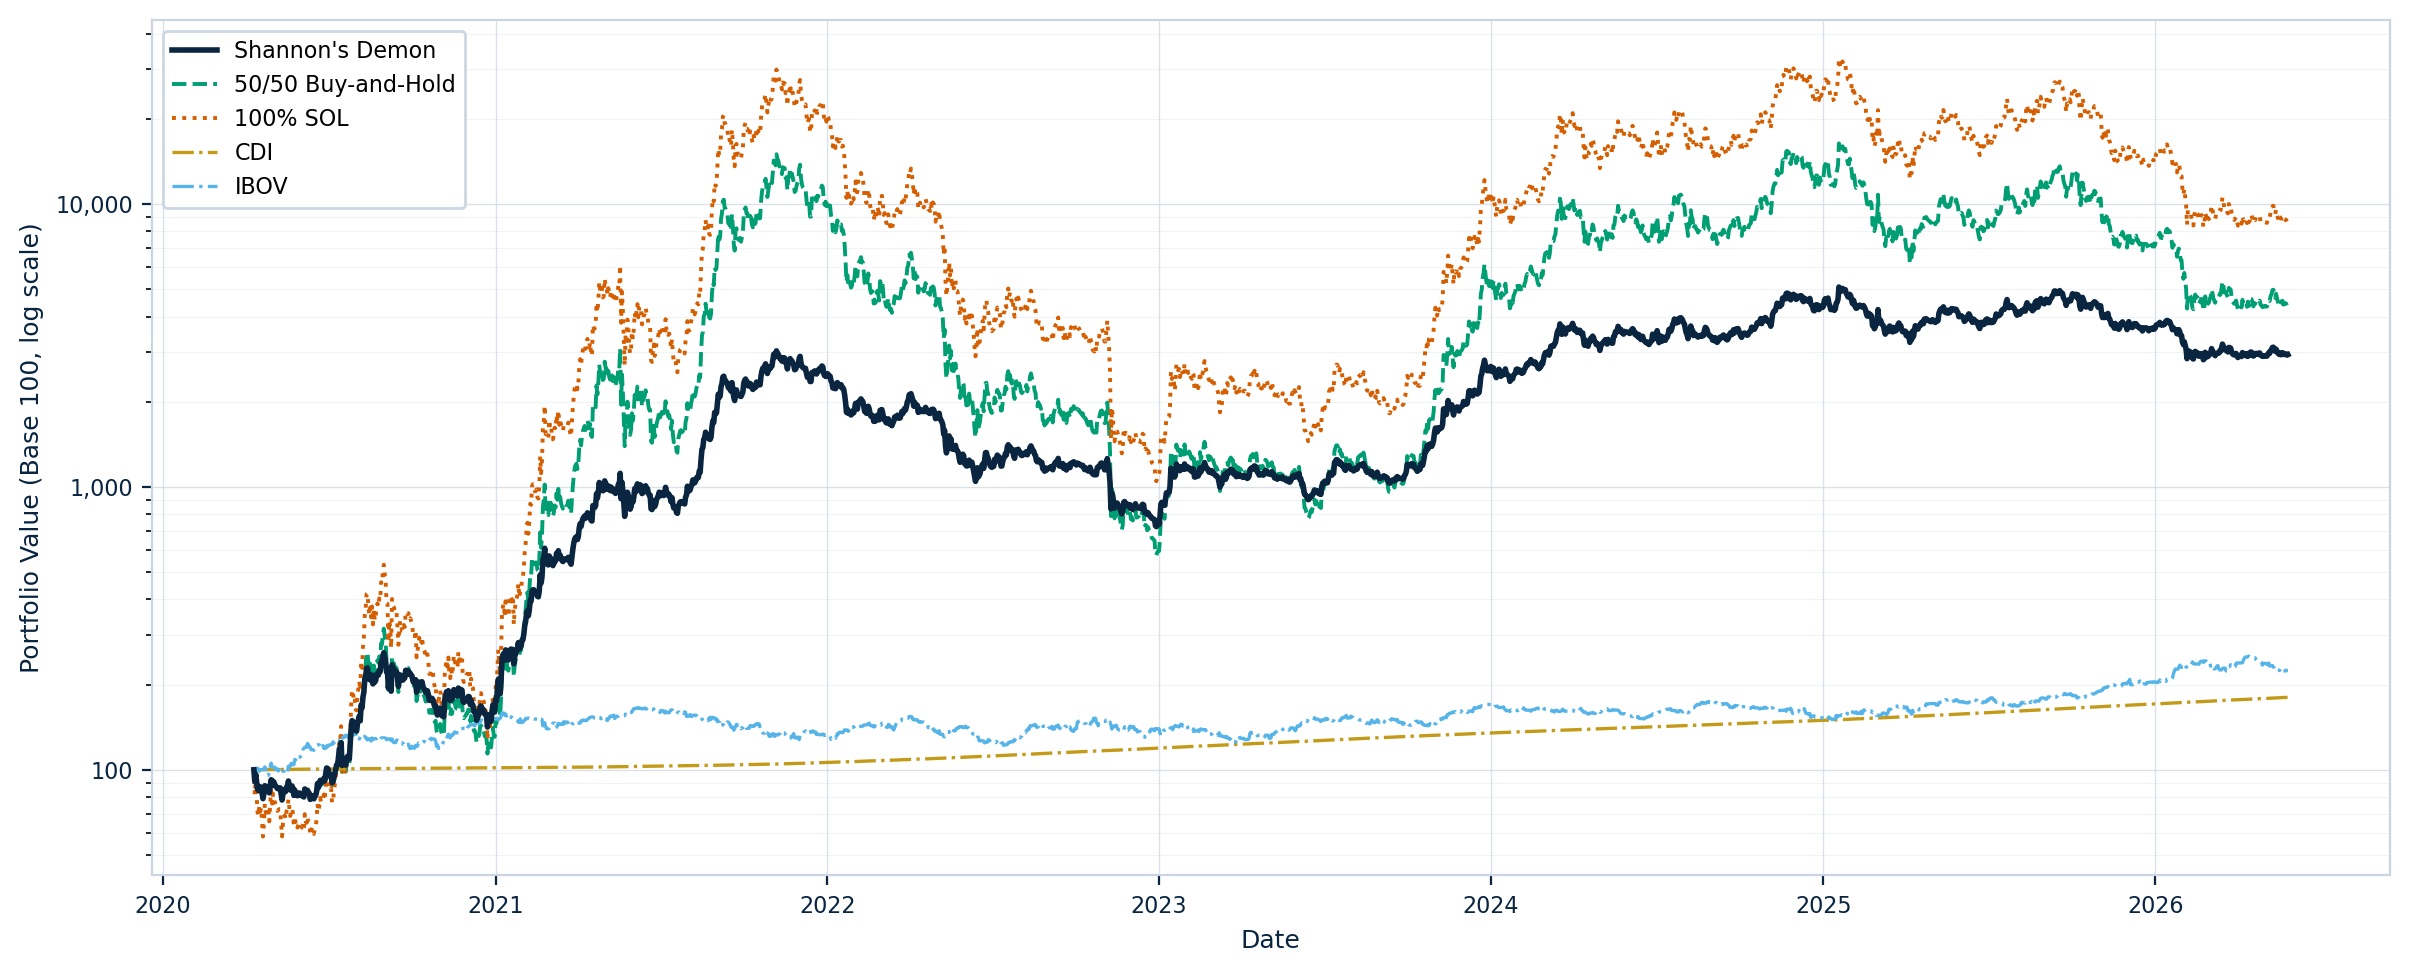
\includegraphics[width=0.97\textwidth,height=0.68\textheight,keepaspectratio]{charts/chart_performance}
\end{center}
\vspace*{\fill}
{\scriptsize\color{MutedText}\itshape
Past performance does not guarantee future results. Backtest from Apr~2020 to May~2026
on simulated portfolio starting at R\$100. Fees of~0.30\% per rebalance applied.
Shannon Capital is not a registered investment adviser. Not financial advice.}
\end{frame}

\begin{frame}{Drawdown from Peak}
\vspace{0.2em}
\begin{center}
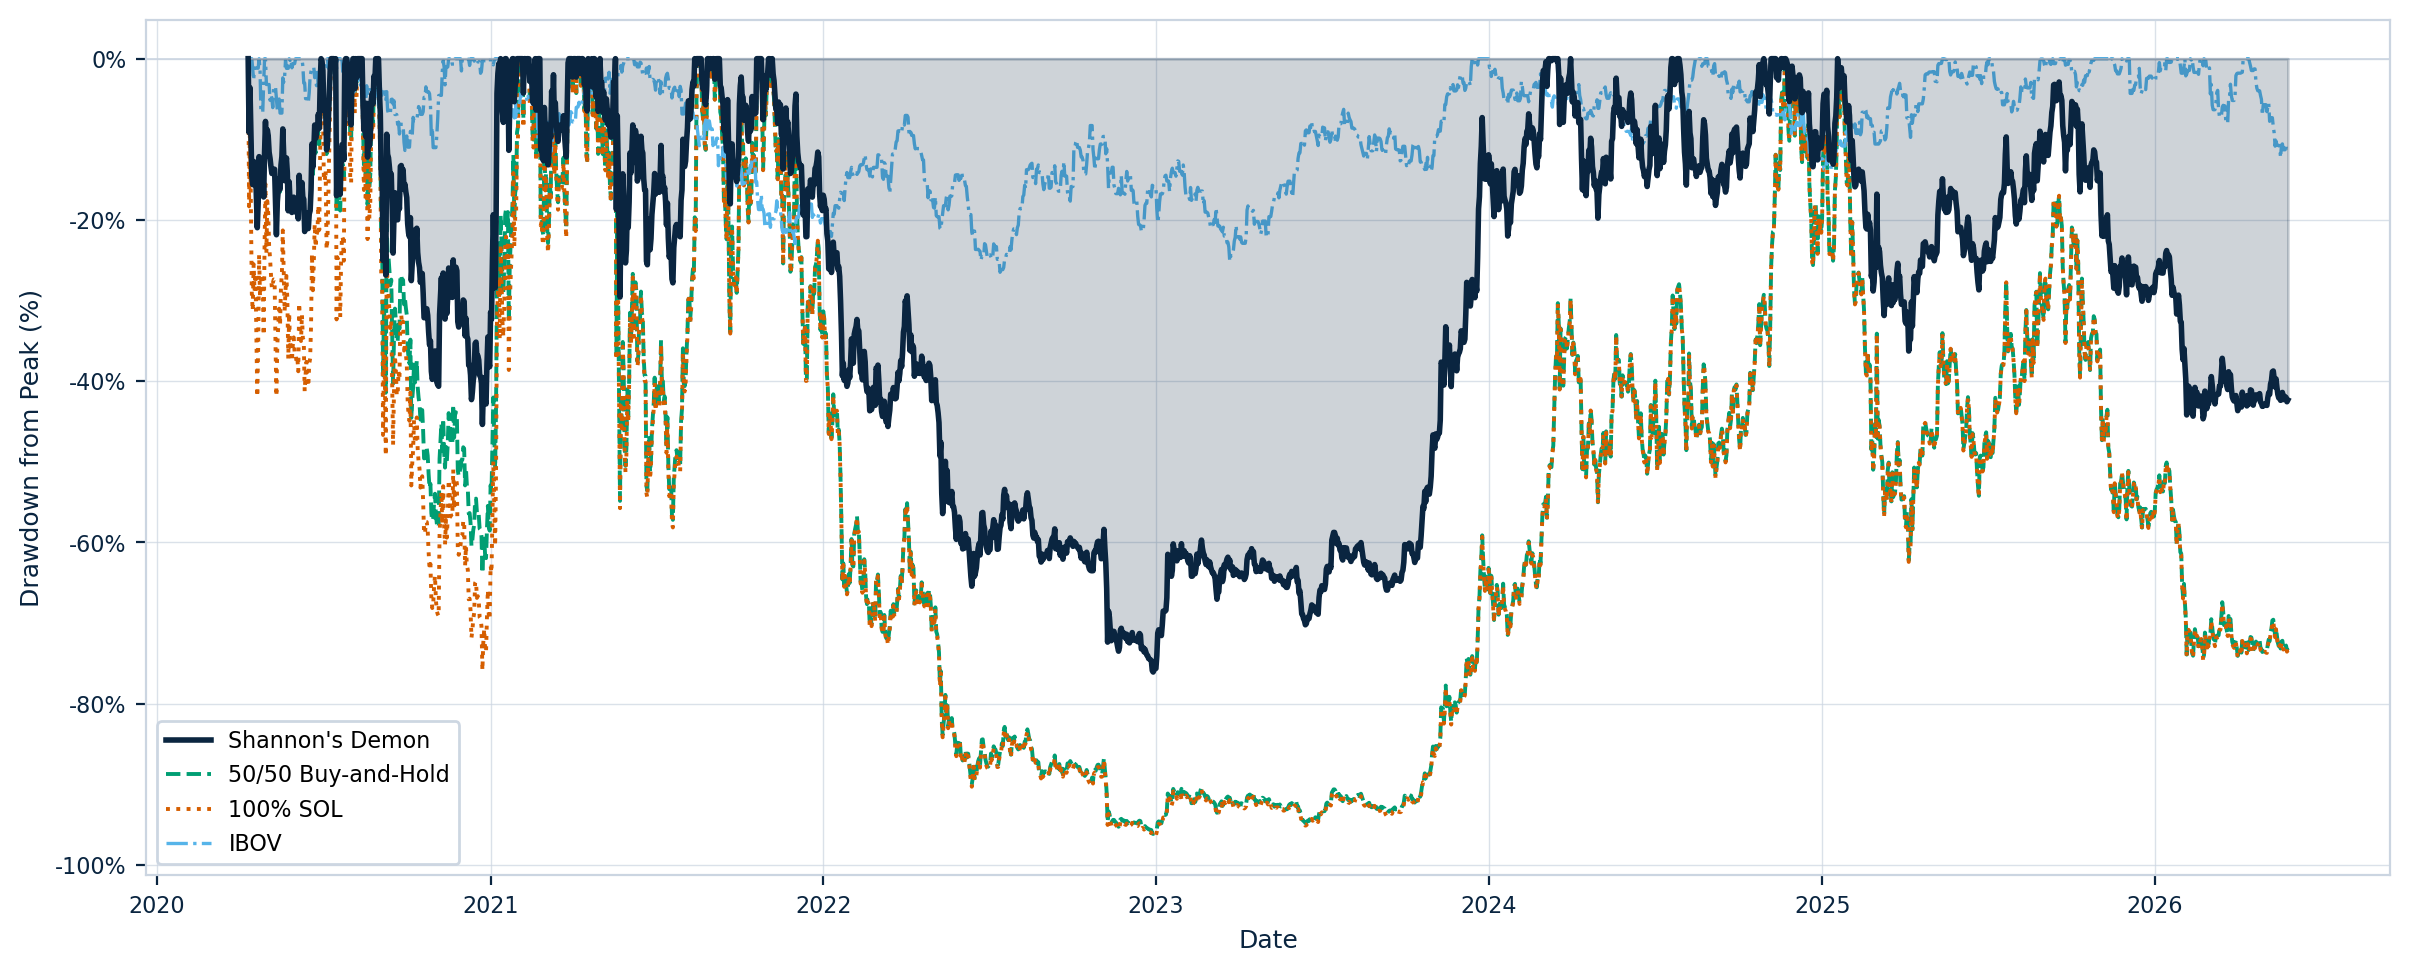
\includegraphics[width=0.97\textwidth,height=0.68\textheight,keepaspectratio]{charts/chart_drawdown}
\end{center}
\vspace*{\fill}
{\scriptsize\color{MutedText}\itshape
Past performance does not guarantee future results. Backtest from Apr~2020 to May~2026
on simulated portfolio starting at R\$100. Fees of~0.30\% per rebalance applied.
Shannon Capital is not a registered investment adviser. Not financial advice.}
\end{frame}

\begin{frame}{Overall Risk Metrics --- Apr 2020 to May 2026}
\vspace{0.2em}
\begin{center}
\arrayrulecolor{RuleColor}
\footnotesize
\begin{tabular}{@{\hspace{0.3em}}l r r r r r@{\hspace{0.3em}}}
\toprule
\rowcolor{Navy}
  \textcolor{white}{\textbf{Metric}} &
  \textcolor{white}{\textbf{Shannon}} &
  \textcolor{white}{\textbf{50/50 B\&H}} &
  \textcolor{white}{\textbf{100\% SOL}} &
  \textcolor{white}{\textbf{CDI}} &
  \textcolor{white}{\textbf{IBOV}} \\
\midrule
Total Return      & \textcolor{Success}{+2{,}833\%}  & \textcolor{Success}{+4{,}298\%}  & \textcolor{Success}{+8{,}596\%}  & \textcolor{Success}{+80.2\%}  & \textcolor{Success}{+124.0\%} \\
Annual Return     & \textcolor{Success}{+46.3\%} & \textcolor{Success}{+53.1\%} & \textcolor{Success}{+65.3\%} & \textcolor{Success}{+6.9\%}  & \textcolor{Success}{+9.5\%}  \\
Annual Volatility & +50.5\% & +90.5\% & +101.4\% & +0.4\% & +15.7\% \\
Sharpe (CDI rf)   & \textbf{0.872} & 0.848 & 0.932 & 0.002 & 0.235 \\
Sortino (CDI rf)  & \textbf{0.884} & 0.566 & 0.650 & 0.000 & 0.195 \\
Max Drawdown      & \textcolor{Danger}{$-$76.1\%} & \textcolor{Danger}{$-$96.2\%} & \textcolor{Danger}{$-$96.5\%} & +0.0\% & \textcolor{Danger}{$-$26.5\%} \\
Final Value (R\$)  & R\$2{,}933 & R\$4{,}398 & R\$8{,}696 & R\$180 & R\$224 \\
Rebalances        & 130 & 0 & 0 & 0 & 0 \\
Total Fees        & R\$40.54 & --- & --- & --- & --- \\
\bottomrule
\end{tabular}
\end{center}
\vspace*{\fill}
{\scriptsize\color{MutedText}\itshape
Past performance does not guarantee future results. Backtest from Apr~2020 to May~2026
on simulated portfolio starting at R\$100. Fees of~0.30\% per rebalance applied.
Shannon Capital is not a registered investment adviser. Not financial advice.}
\end{frame}

\begin{frame}{Yearly Returns by Strategy}
\vspace{0.2em}
\begin{center}
\arrayrulecolor{RuleColor}
\footnotesize
\begin{tabular}{@{\hspace{0.3em}}l r r r r r@{\hspace{0.3em}}}
\toprule
\rowcolor{Navy}
  \textcolor{white}{\textbf{Year}} &
  \textcolor{white}{\textbf{Shannon}} &
  \textcolor{white}{\textbf{50/50 B\&H}} &
  \textcolor{white}{\textbf{100\% SOL}} &
  \textcolor{white}{\textbf{CDI}} &
  \textcolor{white}{\textbf{IBOV}} \\
\midrule
2020 & \textcolor{Success}{+60.16\%} & \textcolor{Success}{+30.76\%} & \textcolor{Success}{+61.51\%} & \textcolor{Success}{+1.63\%} & \textcolor{Success}{+51.33\%} \\
2021 & \textcolor{Success}{+1281.8\%} & \textcolor{Success}{+6512.0\%} & \textcolor{Success}{+9818.1\%} & \textcolor{Success}{+4.42\%} & \textcolor{Danger}{-12.14\%} \\
2022 & \textcolor{Danger}{-70.71\%} & \textcolor{Danger}{-94.25\%} & \textcolor{Danger}{-94.71\%} & \textcolor{Success}{+12.39\%} & \textcolor{Success}{+4.97\%} \\
2023 & \textcolor{Success}{+249.0\%} & \textcolor{Success}{+763.0\%} & \textcolor{Success}{+833.3\%} & \textcolor{Success}{+13.04\%} & \textcolor{Success}{+21.95\%} \\
2024 & \textcolor{Success}{+61.60\%} & \textcolor{Success}{+119.0\%} & \textcolor{Success}{+120.1\%} & \textcolor{Success}{+10.88\%} & \textcolor{Danger}{-10.36\%} \\
2025 & \textcolor{Danger}{-17.17\%} & \textcolor{Danger}{-42.91\%} & \textcolor{Danger}{-43.08\%} & \textcolor{Success}{+14.32\%} & \textcolor{Success}{+33.95\%} \\
2026 & \textcolor{Danger}{-19.46\%} & \textcolor{Danger}{-38.90\%} & \textcolor{Danger}{-39.17\%} & \textcolor{Success}{+5.44\%} & \textcolor{Success}{+9.60\%} \\
\midrule
\textbf{Total} & \textcolor{Success}{+2833\%} & \textcolor{Success}{+4298\%} & \textcolor{Success}{+8596\%} & \textcolor{Success}{+80\%} & \textcolor{Success}{+124\%} \\
\bottomrule
\end{tabular}
\end{center}
\vspace*{\fill}
{\scriptsize\color{MutedText}\itshape
Past performance does not guarantee future results. Backtest from Apr~2020 to May~2026
on simulated portfolio starting at R\$100. Fees of~0.30\% per rebalance applied.
Shannon Capital is not a registered investment adviser. Not financial advice.}
\end{frame}

\begin{frame}{Shannon's Demon --- Monthly Return Calendar}
\vspace{0.2em}
\begin{center}
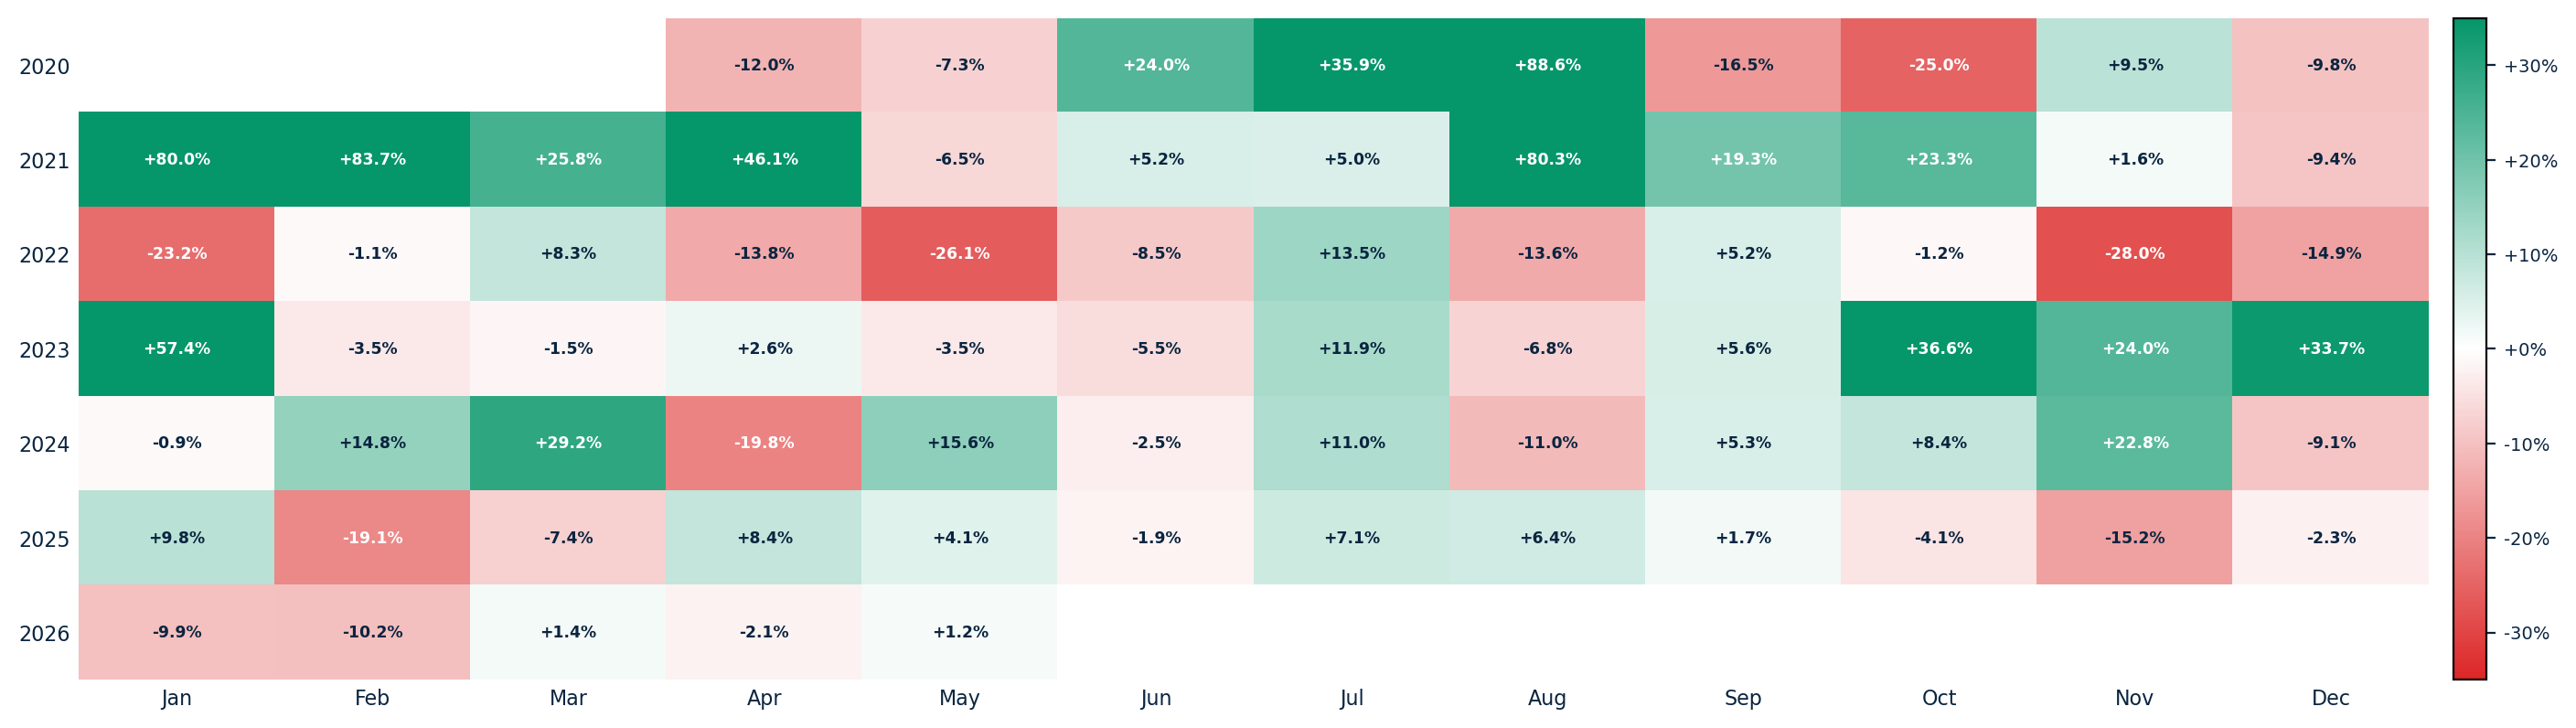
\includegraphics[width=0.97\textwidth,height=0.72\textheight,keepaspectratio]{charts/chart_monthly_heatmap}
\end{center}
{\scriptsize\color{MutedText}\itshape
Color scale clipped at $\pm$35\%; annotated values show actuals.
{\scriptsize\color{MutedText}\itshape
Past performance does not guarantee future results. Backtest from Apr~2020 to May~2026
on simulated portfolio starting at R\$100. Fees of~0.30\% per rebalance applied.
Shannon Capital is not a registered investment adviser. Not financial advice.}}
\end{frame}

\begin{frame}{Performance Across Market Regimes}
\vspace{0.3em}
\arrayrulecolor{RuleColor}
\small
\begin{center}
\begin{tabular}{@{\hspace{0.3em}}l l r r@{\hspace{0.3em}}}
\toprule
\rowcolor{Navy}
  \textcolor{white}{\textbf{Regime}} &
  \textcolor{white}{\textbf{Period}} &
  \textcolor{white}{\textbf{Shannon}} &
  \textcolor{white}{\textbf{50/50 B\&H}} \\
\midrule
\textbf{Bull --- explosive rally} & 2021 & \textcolor{Success}{+1{,}282\%} & \textcolor{Success}{+6{,}512\%} \\
\textbf{Bear --- prolonged crash} & 2022 & \textcolor{Danger}{$-$70.7\%} & \textcolor{Danger}{$-$94.3\%} \\
\textbf{Recovery --- trend up}    & 2023 & \textcolor{Success}{+249\%}   & \textcolor{Success}{+763\%} \\
\textbf{Mixed --- moderate up}    & 2024 & \textcolor{Success}{+61.6\%}  & \textcolor{Success}{+119\%} \\
\textbf{Downturn --- grind down}  & 2025 & \textcolor{Danger}{$-$17.2\%} & \textcolor{Danger}{$-$42.9\%} \\
\bottomrule
\end{tabular}
\end{center}

\vspace{0.3em}
{\small\color{BodyText}
\textbf{Shannon's key advantage:} risk reduction during downturns.
In 2022, the strategy limited losses to $-$70.7\% vs $-$94.3\% for B\&H --- preserving
\textbf{4.0$\times$ more capital} through the bear.
In strong bull markets (2021), buy-and-hold dominates; the strategy sacrifices
upside to earn a better Sharpe and Sortino ratio over the full cycle.}

\vspace*{\fill}
{\scriptsize\color{MutedText}\itshape
Past performance does not guarantee future results. Backtest from Apr~2020 to May~2026
on simulated portfolio starting at R\$100. Fees of~0.30\% per rebalance applied.
Shannon Capital is not a registered investment adviser. Not financial advice.}
\end{frame}

\setbeamercolor{background canvas}{bg=Navy}
\begin{frame}[plain]
\begin{tikzpicture}[remember picture,overlay]
  \fill[Gold] (current page.north west) rectangle ([yshift=-0.18cm]current page.north east);
  \fill[Gold] (current page.south west) rectangle ([yshift=0.09cm]current page.south east);
\end{tikzpicture}
\vspace{2.5cm}
\begin{center}
  {\color{Gold}\small\bfseries SECTION V}\\[0.3cm]
  {\color{Gold}\rule{6cm}{0.6pt}}\\[0.4cm]
  {\color{white}\fontsize{22}{28}\selectfont\bfseries Risk Considerations}
\end{center}
\end{frame}
\setbeamercolor{background canvas}{bg=PageBg}

\begin{frame}{Risk Factors \& Operational Notes}
\vspace{0.3em}
{\small\color{BodyText}
\textbf{Strategy risks:}
\begin{itemize}
  \setlength\itemsep{0.15em}
  \item \textbf{Trending markets:} a sustained directional move locks in losses
        rather than extracting a premium. Shannon underperforms B\&H during strong bull runs.
  \item \textbf{Volatility drought:} low-volatility regimes produce few rebalances
        and the CDI risk premium can turn negative over short windows.
  \item \textbf{Total loss:} SOL could go to zero. The BRL side would remain,
        but the strategy provides no guarantee against full loss of the crypto leg.
\end{itemize}

\vspace{0.3em}
\textbf{Operational risks:}
\begin{itemize}
  \setlength\itemsep{0.15em}
  \item \textbf{Exchange risk:} Mercado Bitcoin platform outages, API failures,
        regulatory action, or insolvency.
  \item \textbf{Order execution:} market orders fill at taker prices.
        Slippage $>$1\% from expected price aborts the cycle.
  \item \textbf{Brazilian tax (Lei 9.250/1995 Art.~21):} SELL proceeds
        $>$R\$35{,}000/month are taxable at 15\%. The bot tracks cumulative
        monthly sales and enforces the exemption limit when configured.
  \item \textbf{Software errors:} crash during order execution may leave
        the portfolio in an unbalanced state until manual recovery.
\end{itemize}
}
\end{frame}

\begin{frame}[allowframebreaks]{Important Disclosures}
\scriptsize
\color{BodyText}
\setlength{\parskip}{0.5em}

\textcolor{Navy}{\textbf{NOT INVESTMENT ADVICE}} \quad
This material has been prepared by Shannon Capital for informational and educational
purposes only. It does not constitute an offer, solicitation, or recommendation to buy
or sell any financial instrument or digital asset. Nothing in this presentation should
be construed as investment, financial, legal, or tax advice.

\textcolor{Navy}{\textbf{PAST PERFORMANCE}} \quad
All backtest results are simulated from historical market data and do not represent
actual trading results. Backtest methodology: daily close prices, simulated market
orders, 0.30\% fee per rebalance, R\$100 starting capital, adaptive threshold
(30-day MAD $\times$ 1.5, clamped [50, 500]~bps). Slippage, partial fills, and
out-of-hours price gaps are not modelled. Past performance does not guarantee future
results. Actual results will differ materially.

\textcolor{Navy}{\textbf{RISK FACTORS}} \quad
This strategy involves investment in highly volatile digital assets. Risks include:
(i)~extreme price volatility and potential total or near-total loss of capital;
(ii)~liquidity risk --- positions may not be exitable at prevailing market prices;
(iii)~no guarantee of positive returns or outperformance of any benchmark;
(iv)~the strategy may significantly underperform a passive buy-and-hold position or
the risk-free rate (CDI) during sustained directional markets;
(v)~operational risks including exchange downtime, API failures, network errors,
and software defects.

\textcolor{Navy}{\textbf{REGULATORY}} \quad
This material has not been reviewed or approved by any regulatory authority
(CVM or otherwise). Shannon Capital is an independent asset manager operating under
Brazilian law. This document does not constitute investment advice within the meaning
of Lei 6.385/1976 or applicable CVM regulations. Recipients should obtain independent
financial, legal, and tax advice before making any investment decision.

\textcolor{Navy}{\textbf{TAX}} \quad
Tax information relating to Lei 9.250/1995 Art.~21 is provided for illustrative
purposes only and does not constitute tax advice. Tax rules may change. Recipients
are solely responsible for their own tax compliance obligations.

\vspace{0.3em}
{\color{MutedText}\textcopyright{} Shannon Capital. Confidential ---
Not for distribution. All rights reserved. Unauthorized reproduction or
redistribution is strictly prohibited.}

\end{frame}

\end{document}